\section*{}
\begin{frame}{}
\begin{beamercolorbox}[colsep=1.5pt,rounded=true,shadow=true]{block body example}
    \huge{Chapter 5: Enabling a positive secrecy gap}
\end{beamercolorbox}
\vspace{2cm}
\textbf{Publications:}\\
 C. Paschou, O. Johnson, A. Doufexi, Z. Zhu, and W.H. Chin. ``Increasing the secrecy gap in quasi-static Rayleigh channels with secret splitting.'' In 2020 IEEE Globecom Workshops (GC Wkshps, pp. 1-7. IEEE, 2020.

\end{frame}

\section{Enabling a positive secrecy gap}


\begin{frame}{Motivation}
\title{How can we achieve confidentiality in non-static environments?}

\begin{itemize}
    \item Limitations of PL key-generation protocols: Slow-fading channels result in a low-key rate;

\item Vulnerability of PL key generation protocols: In directive channels, spatial channel correlation remains high over long distances. The eavesdropper may attain useful information about the key;

\item On the other hand \textbf{keyless PLS} does not rely on the spatial decorrelation property nor a dynamic channel but requires a \textbf{positive secrecy gap};

\end{itemize}
\end{frame}


\begin{frame}{Motivation}
\framesubtitle{The main limitation of keyless PLS}
    
\begin{figure}
\vspace{-1cm}
    \centering
    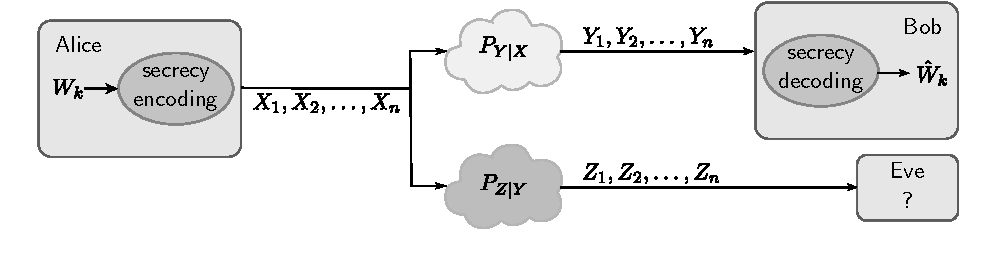
\includegraphics[scale = 0.65]{slides/figures/WiretapChannelCK.pdf}
    \vspace{-.5cm}
    \caption{The generic wiretap channel. Secure transmission is possible only when Bob experiences a better signal quality. I.e. a positive secrecy gap is needed.}
    \label{fig:CK}
\end{figure}
\vspace{-.5cm}
\begin{definition}
    Secrecy gap is the quality difference between the legitimate channel and the wiretap channel. 
\end{definition}

\end{frame}

\begin{frame}{Our solution}
\begin{itemize}
\item Address the requirement of a positive secrecy gap and apply keyless PLS for securely transferring small data such as keys;
\item Our method: Secret splitting utilises user cooperation and significantly increases the probability of a positive secrecy gap.

\end{itemize}. 
\end{frame}

\begin{frame}{Our solution}
\framesubtitle{Related work and differentiation}
The concept of secret splitting has its origins in \textbf{network coding}, but the proposed scheme focuses on using links created solely in the \textbf{physical layer}, particularly in the context of \textbf{distributed massive-MIMO and BS cooperation}.
    
\end{frame}

\begin{frame}{Secret Splitting}
Secret splitting relies on BS cooperation on the downlink and transmit beamforming.
    \framesubtitle{BS cooperation}
    \begin{figure}
        \centering
        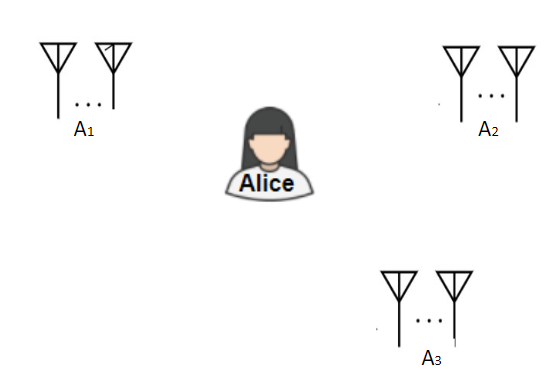
\includegraphics[scale=0.4]{figures/enabling_positive_secrecy_gap/SS_BS_cooperation.png}
        \caption{Alice is able to control two or more base stations.}
    \end{figure}
\end{frame}

\begin{frame}{Secret Splitting}
    \framesubtitle{Main Idea}

    The secret is split in multiple segments.\\
    Eve cannot be close to all transmitting nodes simultaneously. \\
    Eve is unable to reconstruct the secret.
    
    \begin{figure}
        \centering
        \includegraphics[scale=0.4]{figures/enabling_positive_secrecy_gap/SS_channel_model.PNG}
        \caption{Examplar case when Alice deploys two base stations. Bob reveals the secret by XORing the two splits.}
        \label{fig:enter-label}
    \end{figure}
\end{frame}

\begin{frame}{Secret Splitting}
    \framesubtitle{Probability of a positive secrecy gap.}

    \begin{figure}
        \centering
        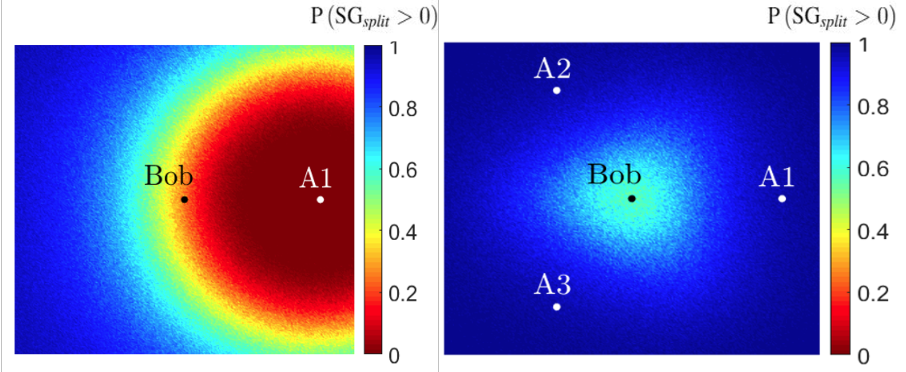
\includegraphics[scale=0.4]{figures/enabling_positive_secrecy_gap/SS_area.PNG}
        \caption{Left: conventional case without BS cooperation\\
        Right: Secret splitting with 3 BSs.}
        \label{fig:enter-label}
    \end{figure}
\end{frame}

\begin{frame}{Insights from Analysis}
\begin{itemize}

\item The secrecy capacity decreases linearly with the number of base stations;
\item Therefore, it is recommended to restrict secret splitting for the confidential transmission of keys;
\item When the total number of antennas is constrained, it is more beneficial to distribute the antennas at two BSs as long as the legitimate receiver is between them;
\item Therefore, the proposed scheme is a good fit for scenarios where the legitimate receiver moves along streets or railways.
\end{itemize}
\end{frame}

\begin{frame}{Concluding remarks}
\begin{itemize}
    \item Secret Splitting dramatically decreases the areas over which the eavesdropper has an advantage over the intended receiver;
    \item I.e., secret splitting enables a positive secrecy gap with a high probability;
    \item Secret splitting is recommended for the secure transmission of keys or other small data. 
\end{itemize}
    
\end{frame}